%%%%%%%%%%%%%%%%%%%%%%%%%%%%%%%%%%%%%%%%%%%%%%%%%%%%%%%%%%%%%%%%%%%%%%%%%%%%%%%%
%                                                                
%                            APÊNDICES                           
%                                                                
% Segundo a NBR 14724 de dezembro de 2005, a diferença primordial entre 
% Anexo e Apêndice é que o Anexo é um texto ou documento não elaborado pelo 
% autor do Trabalho Científico (TC) (monografia, tese, etc.) e o Apêndice é um 
% texto ou documento elaborado pelo autor do TC, ou seja, se foi necessário 
% você criar uma entrevista, um relatório, ou qualquer documento com o escopo 
% de complementar sua argumentação, deve-se utilizar o termo Apêndice e não 
% Anexo. 
% http://www.tudosobremonografia.com/2011/01/diferenca-entre-anexo-e-apendice.html
%%%%%%%%%%%%%%%%%%%%%%%%%%%%%%%%%%%%%%%%%%%%%%%%%%%%%%%%%%%%%%%%%%%%%%%%%%%%%%%%
%                                                                  

\appendix{Derivação do cálculo do gradiente da rede de Elman para modelagem acústica por diferenciação automática} \label{a:equivalencia_fwi_rnn}

  Considere a inversão sísmica de dados obtidos por um receptor, e cujas amplitudes são geradas por uma fonte pontual. Neste contexto, deduziremos o cálculo do gradiente de um modelo de velocidades parametrizado na matriz $\boldsymbol{V}$ utilizando da equação acústica da onda e da função custo de meio erro quadrático $c$ entre as amplitudes modeladas $\hat{y}_t$ e medidas $y_t$ para cada tempo $t$. Desenvolvimentos semelhantes são encontrados nos trabalhos de \shortciteN{richardson2018seismic}, \shortciteN{sun2019deep} e \shortciteN{ren2020physics}. O caso elástico é discutido por \shortciteN{wang2021elastic}. Nos termos descritos, temos:

  \begin{equation} \label{e:custo_rnn}
    c(\boldsymbol{V}) =
    \frac{1}{2} \sum \limits_{t=1}^T e_t^2 =
    \frac{1}{2} \sum \limits_{t=1}^T [\hat{y}_t - y_t]^2 =
    \frac{1}{2} \sum \limits_{t=1}^T
      \left[
        \sum \limits_{\vec{r} \in \mathcal{D}} \delta_{\vec{r}, \vec{r}_r}
        (\boldsymbol{\hat{P}}_t - y_t)
      \right]^2
    ,
  \end{equation}

  \noindent onde $\boldsymbol{\hat{P}}_t$ é o campo modelado no tempo $t$ e $\delta_{\vec{r}, \vec{r}_r}$ é o delta de Kronecker que zera os valores de todos os índices, que não os presentes na posição do receptor $\vec{r}_r$ da matriz à qual é aplicado. Portanto, o somatório da matriz esparsa $\delta_{\vec{r}, \vec{r}_r}(\boldsymbol{\hat{P}}_t - y_t)$ é exatamente o valor do seu único elemento não nulo, $\hat{y}_t - y_t$. Esta escrita facilitará a diferenciação numa etapa posterior. Podemos então diferenciar parcialmente a função custo com relação ao campo de velocidades para calclularmos seu gradiente:

  \begin{equation} \label{e:parcial_custo_wrt_velocidade}
    \frac{\partial c}{\partial \boldsymbol{V}} =
      \sum \limits_{t=1}^T
      \frac{\partial c}{\partial \boldsymbol{\hat{P}}_t} \biggm\lvert_{\boldsymbol{V}}
      \frac{\partial \boldsymbol{\hat{P}}_t}{\partial \boldsymbol{V}} \biggm\lvert_{\boldsymbol{P_{t'\ne t}}}
    .
  \end{equation}

  Por sua vez, num esquema de diferenças finitas de segunda ordem no tempo, $\boldsymbol{\hat{P}}_t$ é dado por:

  \begin{equation} \label{e:fdm_rnn_cell}
    \boldsymbol{\hat{P}}_t =
      \boldsymbol{V}^2 {\Delta t}^2
      (\nabla^2 \boldsymbol{\hat{P}}_{t-1} + s_{t} \boldsymbol{\delta}_{\vec{r}, \vec{r}_s}) +
      2 \boldsymbol{\hat{P}}_{t-1} - 
      \boldsymbol{\hat{P}}_{t-2}
    ,
  \end{equation}

  \noindent onde $\Delta t$ é o menor intervalo de tempo utilizado na modelagem, $s_t$ e $\vec{r}_s$ são respectivamente a amplitude atual e a posição da fonte, e $\boldsymbol{\delta}_{\vec{r}, \vec{r}_s} = \delta_{\vec{r}, \vec{r}_s} \boldsymbol{1}$ é a matriz esparsa cujo único valor não-nulo vale um e se localiza na posição da fonte. Deste modo, função de propagação no tempo pode ser dada por $f$ na equação a seguir:

  \begin{equation} \label{e:fdm_rnn_cell_funcao}
    f(\boldsymbol{V}, \boldsymbol{\hat{P}}_{t-2}, \boldsymbol{\hat{P}}_{t-1}, \boldsymbol{S}) =
      \boldsymbol{V}^2 {\Delta t}^2
      (\nabla^2 \boldsymbol{\hat{P}}_{t-1} + \boldsymbol{S}) +
      2 \boldsymbol{\hat{P}}_{t-1} - 
      \boldsymbol{\hat{P}}_{t-2}
    ,
  \end{equation}

  \noindent onde $\boldsymbol{S}$ é a matriz do termo fonte.

  A diferenciação parcial do custo em relação ao campo de pressão do tempo discreto $t$ na equação \ref{e:parcial_custo_wrt_velocidade} pode ser destrinchada em três \DIFdelbegin \DIFdel{outros termos }\DIFdelend \DIFaddbegin \DIFadd{fatores }\DIFaddend pela regra da cadeia reversa \DIFdelbegin \DIFdel{, uma vez que as }\DIFdelend \DIFaddbegin \DIFadd{(grafo na Figura \ref{f:diferenciando_custo_3_nos}). Isto porque a modelagem por }\DIFaddend diferenças finitas de segunda ordem \DIFdelbegin \DIFdel{fazem }\DIFdelend \DIFaddbegin \DIFadd{no tempo implica }\DIFaddend a propagação de um novo \DIFdelbegin \DIFdel{tempo }\DIFdelend \DIFaddbegin \DIFadd{instante de pressão }\DIFaddend depender de outros \DIFdelbegin \DIFdel{dos campos de outros dois tempos}\DIFdelend \DIFaddbegin \DIFadd{dois dois instantes passados. Desta forma, o custo devido à pressão em um instante $t$ depende não só dele, mas dos outros dois instantes futuros que dependem dele}\DIFaddend , o que num gráfico de diferenciação automática significa que um mesmo nó \DIFaddbegin \DIFadd{de pressão }\DIFaddend é encontrado por três setas\DIFdelbegin \DIFdel{:
}\DIFdelend \DIFaddbegin \DIFadd{. Matematicamente, isto é descrito na tem-se a equação (\ref{e:parcial_custo_wrt_pressao_t_em_v})
}\DIFaddend 

  \DIFaddbegin \begin{figure}
    \begin{center}
      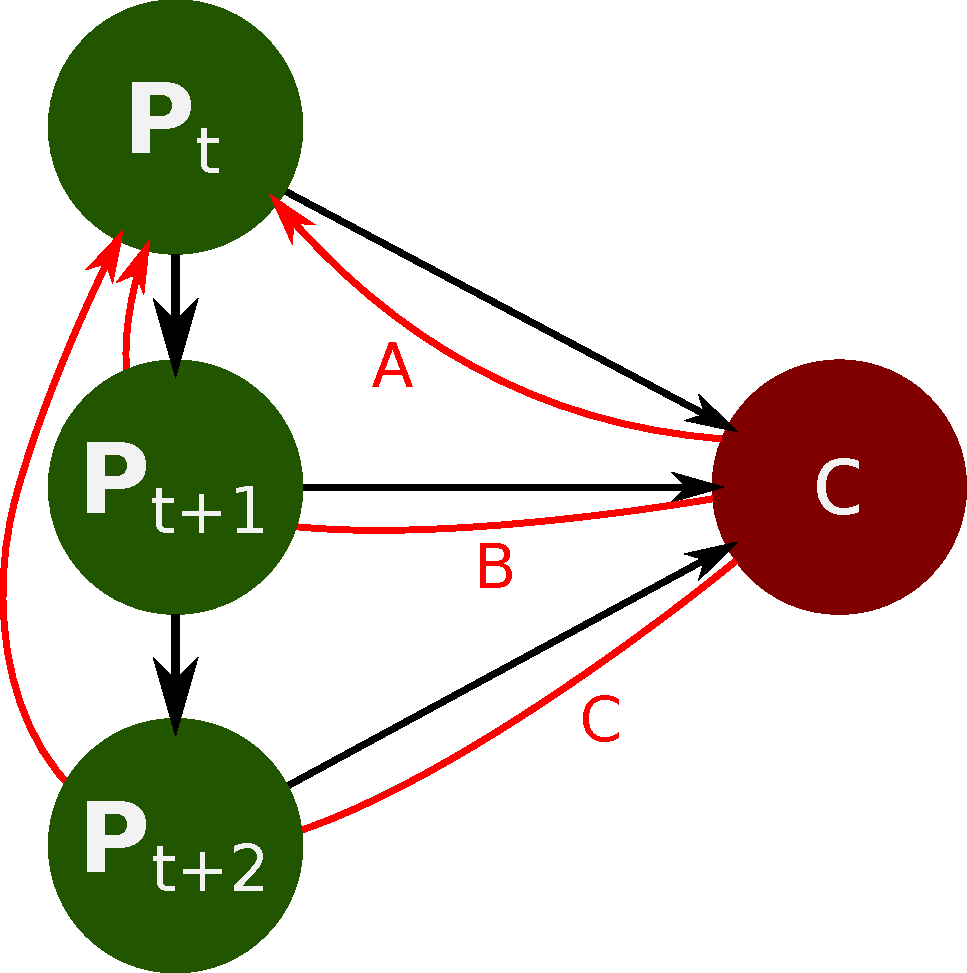
\includegraphics[width=0.3\textwidth]{diferenciando_custo_3_nos.pdf}
    \end{center}
    \caption{\DIFaddFL{Grafo da dependência (setas vermelhas) do custo $c$ em relação ao campo de pressão $P_t$. Num esquema de diferenças finitas de segunda ordem no tempo, três caminhos vão do custo ao campo de pressão em um tempo $t$: o caminho $A$ indica o erro gerado diretamente pela falta de fase entre o dado predito e o observado nos receptores no instante $t$; o caminho $B$ se refere ao erro propagado à pressão do instante seguinte ($t+1$) devido ao erro presente no instante $t$; e o caminho $C$ trata do erro causado à pressão em $t+2$ devido ao erro em $P_t$.}}
    \label{f:diferenciando_custo_3_nos}
  \end{figure}

  \DIFaddend \begin{equation} \label{e:parcial_custo_wrt_pressao_t_em_v}
    \frac{\partial c}{\partial \boldsymbol{\hat{P}}_t} \biggm\lvert_{\boldsymbol{V}} =
    \frac{\partial c}{\partial \boldsymbol{\hat{P}}_t} \biggm\lvert_{\boldsymbol{V}, \boldsymbol{P}_{t'\ne t}} + 
    \frac{\partial c}{\partial \boldsymbol{\hat{P}}_{t+1}} \biggm\lvert_{\boldsymbol{V}}
      \frac{\partial \boldsymbol{\hat{P}}_{t+1}}{\partial \boldsymbol{\hat{P}}_{t}} \biggm\lvert_{\boldsymbol{V}, \boldsymbol{P}_{t'\ne t, t+1}} +
    \frac{\partial c}{\partial \boldsymbol{\hat{P}}_{t+2}} \biggm\lvert_{\boldsymbol{V}}
      \frac{\partial \boldsymbol{\hat{P}}_{t+2}}{\partial \boldsymbol{\hat{P}}_{t}} \biggm\lvert_{\boldsymbol{V}, \boldsymbol{P}_{t'\ne t, t+2}}
    .
  \end{equation}

    O primeiro termo da equação (\ref{e:parcial_custo_wrt_pressao_t_em_v}) pode ser calculado com facilidade a partir da função custo:

  \begin{equation} \label{e:parcial_custo_wrt_pressao_t_em_v_e_t}
    \frac{\partial c}{\partial \boldsymbol{\hat{P}}_t} \biggm\lvert_{\boldsymbol{V}, \boldsymbol{P}_{t'\ne t}} =
    \frac{\partial}{\partial \boldsymbol{\hat{P}}_t}
      \left[\frac{1}{2}
        \sum \limits_{\vec{r} \in \mathcal{D}} \delta_{\vec{r}, \vec{r}_r}
        (\boldsymbol{\hat{P}}_t - y_t)
      \right]^2 \biggm\lvert_{\boldsymbol{V}, \boldsymbol{P}_{t'\ne t}} = 
      \delta_{\vec{r}, \vec{r}_r} (\boldsymbol{\hat{P}}_t - y_t) =
      e_t \boldsymbol{\delta}_{\vec{r}, \vec{r}_r}
    ,
  \end{equation}

  \noindent ou seja, seu valor é a amplitude do resíduo entre o dado modelado e o observado na posição do receptor, $e_t$. As equações (\ref{e:parcial_pressao_t_mais_1_wrt_pressao_t}), (\ref{e:parcial_pressao_t_mais_2_wrt_pressao_t}) e (\ref{e:parcial_pressao_t_wrt_velocidade}) podem ser calculadas a partir de (\ref{e:fdm_rnn_cell}).


  \begin{equation} \label{e:parcial_pressao_t_mais_1_wrt_pressao_t}
    \frac{\partial \boldsymbol{\hat{P}}_{t+1}}{\partial \boldsymbol{\hat{P}}_t} \biggm\lvert_{\boldsymbol{V}, \boldsymbol{P}_{t'\ne t, t+1}} =
    \boldsymbol{V}^2 {\Delta t}^2 \nabla^2 + 2
  \end{equation}

  \begin{equation} \label{e:parcial_pressao_t_mais_2_wrt_pressao_t}
    \frac{\partial \boldsymbol{\hat{P}}_{t+2}}{\partial \boldsymbol{\hat{P}}_t} \biggm\lvert_{\boldsymbol{V}, \boldsymbol{P}_{t'\ne t, t+2}} =
    -1
  \end{equation}

  \begin{equation} \label{e:parcial_pressao_t_wrt_velocidade}
    \frac{\partial \boldsymbol{\hat{P}}_{t}}{\partial \boldsymbol{V}} \biggm\lvert_{\boldsymbol{P}_{t'\ne t}} =
    2 \boldsymbol{V} {\Delta t}^2 (\nabla^2 \boldsymbol{\hat{P}}_{t-1} + 2 s_{t-1} \boldsymbol{\delta}_{\vec{r}, \vec{r}_s})
  \end{equation}

  \DIFdelbegin \DIFdel{Substituíndo }\DIFdelend \DIFaddbegin \DIFadd{Substituindo }\DIFaddend (\ref{e:parcial_custo_wrt_pressao_t_em_v}) em (\DIFdelbegin \DIFdel{\ref{e:parcial_custo_wrt_pressao_t_em_v}}\DIFdelend \DIFaddbegin \DIFadd{\ref{e:parcial_custo_wrt_velocidade}}\DIFaddend ), temos:

  \begin{equation} \label{e:parcial_custo_wrt_velocidade_subs_1}
    \begin{split}
      \frac{\partial c}{\partial \boldsymbol{V}} =
        \sum \limits_{t=1}^T \biggm( &
          \frac{\partial c}{\partial \boldsymbol{\hat{P}}_t} \biggm\lvert_{\boldsymbol{V}, \boldsymbol{P}_{t'\ne t}} \\
        & + \frac{\partial c}{\partial \boldsymbol{\hat{P}}_{t+1}} \biggm\lvert_{\boldsymbol{V}}
                \frac{\partial \boldsymbol{\hat{P}}_{t+1}}{\partial \boldsymbol{\hat{P}}_{t}} \biggm\lvert_{\boldsymbol{V}, \boldsymbol{P}_{t'\ne t, t+1}} \\
        & + \frac{\partial c}{\partial \boldsymbol{\hat{P}}_{t+2}} \biggm\lvert_{\boldsymbol{V}}
                \frac{\partial \boldsymbol{\hat{P}}_{t+2}}{\partial \boldsymbol{\hat{P}}_{t}} \biggm\lvert_{\boldsymbol{V}, \boldsymbol{P}_{t'\ne t, t+2}}
        \biggm)
        2 \boldsymbol{V} {\Delta t}^2 (\nabla^2 \boldsymbol{\hat{P}}_{t-1} + 2 s_{t-1} \boldsymbol{\delta}_{\vec{r}, \vec{r}_s})
    \end{split}
    .
  \end{equation}

  \DIFdelbegin \DIFdel{Substituíndo }\DIFdelend \DIFaddbegin \DIFadd{Sobrepondo }\DIFaddend então (\DIFdelbegin \DIFdel{\ref{e:parcial_custo_wrt_pressao_t_em_v}}\DIFdelend \DIFaddbegin \DIFadd{\ref{e:parcial_custo_wrt_pressao_t_em_v_e_t}}\DIFaddend ), (\ref{e:parcial_pressao_t_mais_1_wrt_pressao_t}) e (\ref{e:parcial_pressao_t_mais_2_wrt_pressao_t}) \DIFdelbegin \DIFdel{em }\DIFdelend \DIFaddbegin \DIFadd{a }\DIFaddend (\ref{e:parcial_custo_wrt_velocidade_subs_1}), conseguimos:

  \begin{equation} \label{e:parcial_custo_wrt_velocidade_subs_2}
    \begin{split}
      \frac{\partial c}{\partial \boldsymbol{V}} = 
      \sum \limits_{t=1}^T \biggm( &
        e_t \boldsymbol{\delta}_{\vec{r}, \vec{r}_r}
        + (\boldsymbol{V}^2 {\Delta t}^2 \nabla^2 + 2) \frac{\partial c}{\partial \boldsymbol{\hat{P}}_{t+1}} \biggm\lvert_{\boldsymbol{V}}
        - \frac{\partial \boldsymbol{\hat{P}}_{t+2}}{\partial \boldsymbol{\hat{P}}_{t}} \biggm\lvert_{\boldsymbol{V}, \boldsymbol{P}_{t'\ne t, t+2}}
      \biggm) \\
      & 2 \boldsymbol{V} {\Delta t}^2 (\nabla^2 \boldsymbol{\hat{P}}_{t-1} + 2 s_{t-1} \boldsymbol{\delta}_{\vec{r}, \vec{r}_s})
    \end{split}
    ,
  \end{equation}

  Podemos rearrumar os termos de (\DIFdelbegin \DIFdel{\ref{e:parcial_custo_wrt_velocidade_subs_1}}\DIFdelend \DIFaddbegin \DIFadd{\ref{e:parcial_custo_wrt_velocidade_subs_2}}\DIFaddend ) da seguinte maneira:

  \begin{equation} \label{e:parcial_custo_wrt_velocidade_rearrumado_2}
    \DIFdelbegin %DIFDELCMD < \begin{split}
%DIFDELCMD <       \frac{\partial c}{\partial \boldsymbol{V}} =
%DIFDELCMD <       \sum \limits_{t=1}^T \biggm(
%DIFDELCMD <         & \boldsymbol{V}^2 {\Delta t}^2 \left(
%DIFDELCMD <           \nabla^2 \frac{\partial c}{\partial \boldsymbol{\hat{P}}_{t+1}} \biggm\lvert_{\boldsymbol{V}} + \frac{e_t \boldsymbol{\delta}_{\vec{r}, \vec{r}_r}}{\boldsymbol{V}^2 {\Delta t}^2}
%DIFDELCMD <         \right) + 2 \frac{\partial c}{\partial \boldsymbol{\hat{P}}_{t+1}} \biggm\lvert_{\boldsymbol{V}}) -
%DIFDELCMD <         \frac{\partial c}{\partial \boldsymbol{\hat{P}}_{t+2}} \biggm\lvert_{\boldsymbol{V}}
%DIFDELCMD <       \biggm) \\
%DIFDELCMD <       & 2 \boldsymbol{V} {\Delta t}^2 (\nabla^2 \boldsymbol{\hat{P}}_{t-1} + 2 s_{t-1} \boldsymbol{\delta}_{\vec{r}, \vec{r}_s})
%DIFDELCMD <     \end{split}%%%
\DIFdelend \DIFaddbegin \begin{split}
      \frac{\partial c}{\partial \boldsymbol{V}} =
      \sum \limits_{t=1}^T \biggm(
        & \boldsymbol{V}^2 {\Delta t}^2 \left(
          \nabla^2 \frac{\partial c}{\partial \boldsymbol{\hat{P}}_{t+1}} \biggm\lvert_{\boldsymbol{V}} + \frac{e_t \boldsymbol{\delta}_{\vec{r}, \vec{r}_r}}{\boldsymbol{V}^2 {\Delta t}^2}
        \right) + 2 \frac{\partial c}{\partial \boldsymbol{\hat{P}}_{t+1}} \biggm\lvert_{\boldsymbol{V}} -
        \frac{\partial c}{\partial \boldsymbol{\hat{P}}_{t+2}} \biggm\lvert_{\boldsymbol{V}}
      \biggm) \\
      & 2 \boldsymbol{V} {\Delta t}^2 (\nabla^2 \boldsymbol{\hat{P}}_{t-1} + 2 s_{t-1} \boldsymbol{\delta}_{\vec{r}, \vec{r}_s})
    \end{split}\DIFaddend 
    .
  \end{equation}

  \noindent \DIFdelbegin \DIFdel{Podemos enxergar }\DIFdelend \DIFaddbegin \DIFadd{Enxergamos }\DIFaddend em (\ref{e:parcial_custo_wrt_velocidade_rearrumado_2}) o padrão da função de modelagem $f$ no primeiro fator do somatório:

  \begin{equation} \label{e:parcial_custo_wrt_velocidade_propagacao_reversa}
    \frac{\partial c}{\partial \boldsymbol{V}} =
    \sum \limits_{t=1}^T
    f\left(\boldsymbol{V},
      \frac{\partial c}{\partial \boldsymbol{\hat{P}}_{t+2}} \biggm\lvert_{\boldsymbol{V}}, \frac{\partial c}{\partial \boldsymbol{\hat{P}}_{t+1}} \biggm\lvert_{\boldsymbol{V}}, \frac{e_t \boldsymbol{\delta}_{\vec{r}, \vec{r}_r}}{\boldsymbol{V} {\Delta t}^2}
    \right)
    2 \boldsymbol{V} {\Delta t}^2 (\nabla^2 \boldsymbol{\hat{P}}_{t-1} + 2 s_{t-1} \boldsymbol{\delta}_{\vec{r}, \vec{r}_s})
    .
  \end{equation}

  Já no segundo fator de (\ref{e:parcial_custo_wrt_velocidade_rearrumado_2}) podemos ver a segunda derivada do campo primário, uma vez que:

  \begin{equation} \label{e:de_volta_das_diferencas_finitas_para_segunda_derivada_analitica}
    \frac{\boldsymbol{\hat{P}}_t - 2 \boldsymbol{\hat{P}}_{t-1} + \boldsymbol{\hat{P}}_{t-2}}{{\Delta t}^2}
    \approx
    \boldsymbol{\ddot{\hat{P}}}_{t-1}
    =
    \boldsymbol{V}^2 (\nabla^2 \boldsymbol{\hat{P}}_{t-1} + s_{t-1} \boldsymbol{\delta}_{\vec{r}, \vec{r}_s})
    ,
  \end{equation}

  \noindent e portanto,

  \begin{equation} \label{e:segundo_fator_vem_da_segunda_derivada_no_tempo}
    \nabla^2 \boldsymbol{\hat{P}}_{t-1} + s_{t-1} \boldsymbol{\delta}_{\vec{r}, \vec{r}_s}
    =
    \frac{\boldsymbol{\ddot{\hat{P}}}_{t-1}}{\boldsymbol{V}^2}
    .
  \end{equation}

  \noindent Ficamos então com (\ref{e:parcial_custo_wrt_velocidade_propagacao_reversa_com_dt}).

  \begin{equation} \label{e:parcial_custo_wrt_velocidade_propagacao_reversa_com_dt}
    \frac{\partial c}{\partial \boldsymbol{V}} =
    \sum \limits_{t=1}^T
    f\left(\boldsymbol{V},
      \frac{\partial c}{\partial \boldsymbol{\hat{P}}_{t+2}} \biggm\lvert_{\boldsymbol{V}}, \frac{\partial c}{\partial \boldsymbol{\hat{P}}_{t+1}} \biggm\lvert_{\boldsymbol{V}}, \frac{e_t \boldsymbol{\delta}_{\vec{r}, \vec{r}_r}}{\boldsymbol{V} {\Delta t}^2}
    \right)
    \frac{2}{\boldsymbol{V}} {\Delta t}^2 \boldsymbol{\ddot{\hat{P}}}_{t-1}
  \end{equation}

  Dada a linearidade da equação da onda a tempos pequenos, podemos por para fora os fatores do terceiro argumento de $f$ e mover as variáveis independentes do tempo para fora do somatório para obter (\ref{e:parcial_custo_wrt_velocidade_propagacao_reversa_final}).

  \begin{equation} \label{e:parcial_custo_wrt_velocidade_propagacao_reversa_final}
    \boldsymbol{\nabla} c \equiv \frac{\partial c}{\partial \boldsymbol{V}} =
    \frac{2}{\boldsymbol{V}^3}
    \sum \limits_{t=1}^T
    f\left(\boldsymbol{V},
      \frac{\partial c}{\partial \boldsymbol{\hat{P}}_{t+2}} \biggm\lvert_{\boldsymbol{V}}, \frac{\partial c}{\partial \boldsymbol{\hat{P}}_{t+1}} \biggm\lvert_{\boldsymbol{V}}, e_t \boldsymbol{\delta}_{\vec{r}, \vec{r}_r}
    \right)
    \boldsymbol{\ddot{\hat{P}}}_{t-1}
  \end{equation}

  A equação (\ref{e:parcial_custo_wrt_velocidade_propagacao_reversa_final}) é exatamente a discretização da solução para o gradiente da função custo do erro quadrático dada pelo método adjunto: \DIFdelbegin \DIFdel{A }\DIFdelend \DIFaddbegin \DIFadd{a }\DIFaddend função $f$ está propagando o resíduo $e_t$ reversamente no tempo --- a extrapolação vai \DIFdelbegin \DIFdel{dos }\DIFdelend \DIFaddbegin \DIFadd{do }\DIFaddend tempo $t+2$ para $t+1$ para \DIFaddbegin \DIFadd{sem seguida }\DIFaddend produzir $t$ --- a partir da posição do receptor, $\vec{r}_r$. O resultado desta operação é o campo adjunto do método adjunto, $\lambda$, que é multiplicado pela segunda derivada no tempo do campo modelado. Este resultado \DIFdelbegin \DIFdel{, com }\DIFdelend \DIFaddbegin \DIFadd{para }\DIFaddend uma única fonte é \DIFdelbegin \DIFdel{extendido }\DIFdelend \DIFaddbegin \DIFadd{estendido }\DIFaddend a mais receptores somando suas contribuições na função custo, e a mais fontes, ao realizar a modelagem direta com mais fontes \shortcite{sun2019deep}.


\DIFdelbegin %DIFDELCMD < \appendix{Receita para o treinamento estocástico de um modelo supervisionado ou não-supervisionado} %%%
\DIFdelend \DIFaddbegin \appendix{Receita para o treinamento estocástico de um modelo supervisionado} \DIFaddend \label{a:guia_treinamento}

    Durante os estudos práticos \DIFdelbegin \DIFdel{, o }\DIFdelend \DIFaddbegin \DIFadd{de treinamento de modelos supervisionados, tais como o do modelo de regressão logística, a inversão de forma completa da onda implementada, o }\DIFaddend autor verificou um padrão estrutural \DIFdelbegin \DIFdel{durante }\DIFdelend \DIFaddbegin \DIFadd{para }\DIFaddend a implementação de códigos de otimização em um paradigma fortemente funcional, de \DIFdelbegin \DIFdel{forma que os resultados são }\DIFdelend \DIFaddbegin \DIFadd{maneira que os códigos se tornam }\DIFaddend mais facilmente reutilizáveis. Tal padrão pode ser \DIFaddbegin \DIFadd{utilizado para o desenvolvimento de qualquer modelo estatístico supervisionado ou de qualquer inversão geofísica, e é }\DIFaddend sumarizado em três fases:

    \begin{enumerate}
      \item Fase de \emph{criação do modelo}, a qual envolve:
        \begin{enumerate}
          \item Definição do(s) modelo(s) direto(s) --- durante esta etapa deve-se implementar os problemas diretos necessários que levarão uma sequência de parâmetros $\{W_s\}$ e uma matriz de amostras observadas $\boldsymbol{X}$ a uma matriz de predições $\boldsymbol{\hat{Y}}$. Este processo muitas vezes inclui o primeiro desenvolvimento de modelos que levam uma única amostra $\vec{x}$ à sua predição $\vec{y}$.
          \item Em caso de otimização conjunta de dois ou mais modelos diretos deve-se implementar um modelo amarrador que retorna as saídas finais que podem ser utilizadas no treinamento.
          \item Em caso de regularização dos parâmetros durante treinamento, pode ser desejável adicionar os parâmetros como saídas do modelo final utilizado no treinamento.
        \end{enumerate}
      \item Fase de \emph{preparação do treinamento}, que nos termos aqui descritos só faz sentido para numa abordagem funcional. Caso se utilize uma abordagem imperativa, pular à próxima fase. Suas etapas são:
        \begin{enumerate}
          \item Preparação dos dados a serem utilizados no treinamento, incluíndo a estrutura de observações $\boldsymbol{X}$ e estrutura \DIFdelbegin \DIFdel{com }\DIFdelend \DIFaddbegin \DIFadd{de }\DIFaddend seus alvos $\boldsymbol{Y}$ caso aplicável.
          \item Preparação do método de validação (\textit{i.e.}, \textit{holdout}, \textit{k-fold}).
          \item Definição da função custo de erro médio $C(\{\boldsymbol{W}_s\}, \boldsymbol{X}_b, \boldsymbol{Y}_b)$\DIFdelbegin \DIFdel{(lote de observações e de alvos)}\DIFdelend , que toma \DIFdelbegin \DIFdel{um lote de predições e }\DIFdelend \DIFaddbegin \DIFadd{os parâmetros, o lote de dados e seus alvos, e }\DIFaddend retorna um valor em $\mathcal{R}$. Frequentemente inclui-se aqui a definição anterior do custo calculado sobre uma única amostra, $c_n(\{\boldsymbol{W}_s\}, \vec{x}, \vec{y})$.
          \item Opcional: pode-se definir uma função para calcular outras métricas úteis \DIFaddbegin \DIFadd{(}\textit{\DIFadd{i.e.}}\DIFadd{, precisão, acurácia, além do custo) }\DIFaddend a partir de um lote de predições, $\boldsymbol{\hat{Y}}$, e seus valores verdadeiros, $\boldsymbol{Y}$.
          \item Implementação do funcional que toma um modelo, uma função custo médio e, se aplicável, parâmetros da regularização de parâmetros utilizada (\textit{i.e.}\DIFaddbegin \DIFadd{, }\DIFaddend coeficiente do termo de esparsidade dos parâmetros na função custo), e define uma função para calcular o custo $C$ e o gradiente do custo $\nabla C$ deste modelo com relação aos parâmetros dados, \DIFaddbegin \DIFadd{por diferenciação automática, }\DIFaddend partindo deles e de um lote de dados composto por $\boldsymbol{X}_b$ e $\boldsymbol{Y}_b$, caso aplicável. Eventualmente pode ser interessante retornar também nesta função as métricas avaliadas em treinamento por meio de uma função previamente definida, desde que isto não adicione complexidade significativa ao algoritmo de treinamento e haja tempo o suficiente para tal.
          \item Criação de um funcional que toma o modelo e uma função custo para produzir uma função que toma parâmetros e um lote de dados, e retorna suas predições, custo e outras métricas, caso definidas.
          \item Criação de um funcional que toma uma função custo e retorna uma função que treina o modelo por uma época. Para tal, esta função deve recebe um otimizador (\textit{i.e.}, SGD)  com suas variáveis de estado, o lote total de dados a ser utilizado no treinamento, o número de amostras a ser utilizada no treinamento estocástico, e se desejado, uma chave para realizar acumulação de gradientes ou não. A função gerada retornará em cada aplicação pelo menos os parâmetros atualizados após uma época, as novas variáveis de estado do otimizador e as métricas médias obtidas nesta mesma época.
        \end{enumerate}
      \item Fase de \emph{treinamento}, a qual inclui:
        \begin{enumerate}
          \item A geração das funções --- \DIFdelbegin \DIFdel{caso na abordagem funcional, utilizar }\DIFdelend \DIFaddbegin \DIFadd{aplicar }\DIFaddend os funcionais implementados no passo anterior:
            \begin{enumerate}
              \item de treinamento de uma época em função de um otimizador, dados de treinamento, número de amostras por lote e, se desejado, uma opção para acumular gradientes ou não;
              \item de avalização das métricas do modelo.
            \end{enumerate}
          \item Inicializar o otimizador escolhido (\textit{i.e.}, SGD).
          \item Definir uma condição de parada, como a descrita na Seção \ref{s:interrupcao_precoce} ou número máximo de épocas --- não recomendado, pois este parâmetro é difícil de ser escolhido.
          \item Definir uma estrutura de dados para o guardar um histórico de métricas de treinamento.
          \item Criar o laço de treinamento, que tipicamente envolve:
            \begin{enumerate}
              \item treinar uma época;
              \item imprimir \DIFaddbegin \DIFadd{o }\DIFaddend estado do treinamento (\textit{i.e.}, época e valor do custo \DIFaddbegin \DIFadd{atual}\DIFaddend );
              \item atualizar histórico com as métricas atuais;
              \item criar \textit{checkpoint} do modelo --- isto é, salvar seus parâmetros em uma estrutura (tipicamente em disco);
              \item atualizar da condição de parada a partir da métrica avaliada e dos parâmetros atuais;
              \item verificar se a condição de parada retorna verdadeiro. Caso positivo, recuperar \DIFaddbegin \DIFadd{o }\DIFaddend \textit{checkpoint} dos melhores parâmetros do modelo e finalizar treinamento.
            \end{enumerate}
          \item Visualizar saídas do modelo.
          \item Visualizar histórico de métricas salvo\DIFaddbegin \DIFadd{, verificar condições de viés e variância para considerar situações de subajuste ou sobreajuste}\DIFaddend .
          \item Salvar parâmetros do modelo treinado.
        \end{enumerate}
    \end{enumerate}

    Além dos passos apontados acima, vale ressaltar que os parâmetros do otimizador, como a taxa de aprendizado, ou os parâmetros da função custo, como os relacionados à regularização do modelo, devem ser testados para que possam ser \DIFdelbegin \DIFdel{escolhidos}\DIFdelend \DIFaddbegin \DIFadd{definidos}\DIFaddend .


\appendix{Transformação \textit{one-hot}} \label{a:one_hot}

  A transformação ou codificação \textit{one-hot} consiste numa simples transformação rótulos inteiros em probabilidades de pertencimento a cada classe. Assim, se um problema considera que amostras podem pertencer a três classes, enumeradas de 1 a 3, o rótulo 1 se torna $[1.0,\ 0.0,\ 0.0]^\top$, o rótulo 2 se torna $[0.0,\ 1.0,\ 0.0]^\top$, e o rótulo 3 se torna $[0.0,\ 0.0,\ 1.0]^\top$, onde cada linha $i$ destes vetores diz respeito à probabilidade de pertencimento da amostra à classe $i$.

  Geralmente esta aplicação é realizada em massa para um vetor de $N$ rótulos, $\vec{r}$, o qual é associado a uma matriz de observações das $N$ amostras $\boldsymbol{X}_{N\times M}$. O resultado deste processo é uma matriz $\boldsymbol{Y}$ cujas linhas são dadas pela transposta da transformação \textit{one-hot} das linhas em $\vec{r}$. Isto pode ser verificado no caso abaixo:

  \begin{equation}
    \text{one-hot} \left(
    \begin{bmatrix}
      1 \\
      2 \\
      2 \\
      3
    \end{bmatrix} \right)
    =
    \begin{bmatrix}
      1.0 & 0.0 & 0.0 \\
      0.0 & 1.0 & 0.0 \\
      0.0 & 1.0 & 0.0 \\
      0.0 & 0.0 & 1.0 \\
    \end{bmatrix}
    .
  \end{equation}

  A transformação one-hot pode ser invertida aplicando a função de argumento do máximo (argmax) em cada linha da matriz transformada. Esta função retorna o índice do elemento com maior valor do vetor aplicado:

  \begin{equation}
    \text{argmax} \left(
    \begin{bmatrix}
      1.0 & 0.0 & 0.0 \\
      0.0 & 1.0 & 0.0 \\
      0.0 & 1.0 & 0.0 \\
      0.0 & 0.0 & 1.0 \\
    \end{bmatrix} \right)
    =
    \begin{bmatrix}
      1 \\
      2 \\
      2 \\
      3
    \end{bmatrix}
    .
  \end{equation}

\appendix{Código para diferenciação automática direta} \label{a:autodiff_direta}

  Este código implementa um ambiente de diferenciação automática direta na linguagem Python 3.9 de forma simples, sem o uso de bibliotecas externas. Ele não deve ser considerado em aplicações com alta demanda computacional, uma vez que foi escrito com fins didáticos.

  \lstinputlisting[language=Python]{code/forward_mode.py}


\appendix{Código para diferenciação automática reversa} \label{a:autodiff_reversa}

  Este código implementa um ambiente de diferenciação automática reversa na linguagem Python 3.9 de forma simples, sem o uso de bibliotecas externas. Ele não deve ser considerado em aplicações com alta demanda computacional, uma vez que foi escrito com fins didáticos. Uma aplicação desta implementação pode ser vista no Apêndice \ref{a:treinamento_mlp}, onde uma rede neural tipo perceptron multicamadas é treinada.

  \lstinputlisting[language=Python]{code/reverse_mode.py}


\appendix{Código para treinamento de rede neural MLP usando diferenciação automática} \label{a:treinamento_mlp}

  Este código escrito em Python 3.9 importa o código presente no Apêndice \ref{a:autodiff_reversa} para realizar o cálculo de gradientes por meio da diferenciação automática reversa, qual é utilizado no treinamento de uma rede perceptron multicamadas sem o uso de bibliotecas externas. O algoritmo de otimização utilizado é o SGD.

  \lstinputlisting[language=Python]{code/mlp.py}
